For the online problem we have identified and modeled the following radom variables.
\subsection*{Daily customers distribution}
We modeled the daily customers distribution as a \textbf{Gaussian Distribution}, with a normalizing factor of 1000 daily customers. Average and variance of the Gaussian distribution are reported in the table below.\\
\vspace{3cm}
\begin{tabularx}{0.8\textwidth} { 
		| >{\raggedright\arraybackslash}X 
		| >{\centering\arraybackslash}X 
		| >{\raggedleft\arraybackslash}X | }
	\hline
	Customer Category & Average & Variance  \\
	\hline
	Sport addicted & 0.15 & 0.03  \\
	\hline
	Gifter & 0.20 & 0.03  \\
	\hline
	Worried & 0.40 & 0.05  \\
	\hline
	Amateur & 0.25 & 0.04  \\
	\hline
\end{tabularx}

\begin{center}
	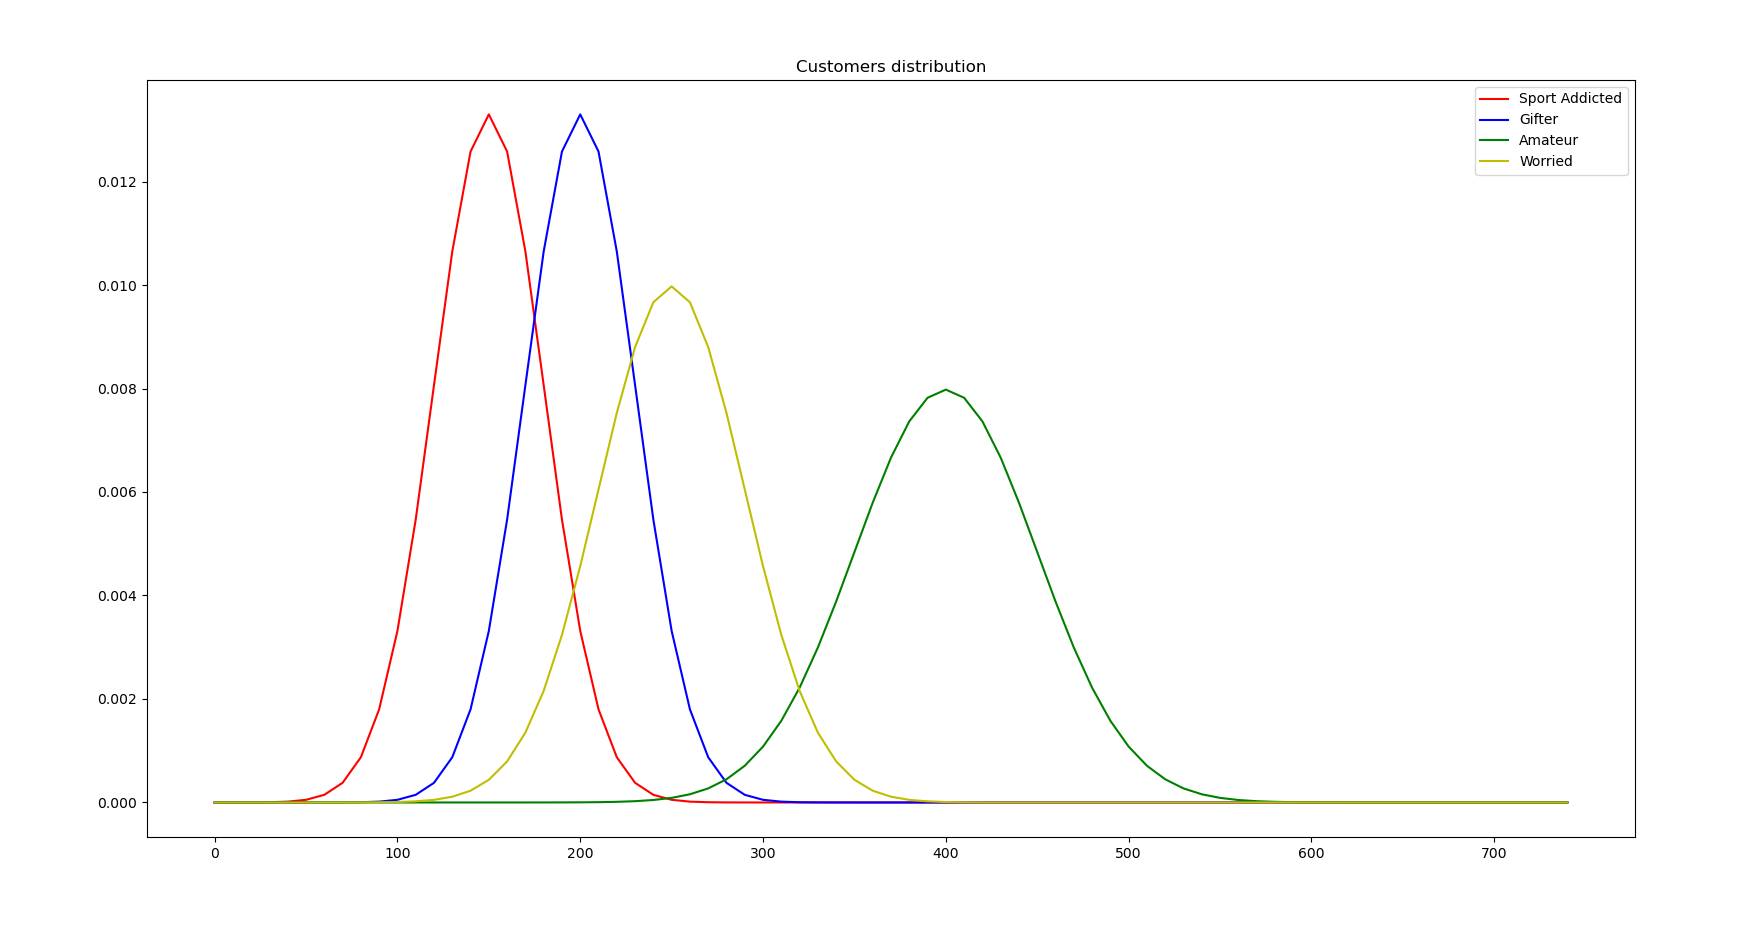
\includegraphics[scale=0.35]{Images/CustomerDistribution}
\end{center}

\subsection*{Conversions rates}
The odds of buying one item are modelled with a \textbf{Bernulli Distribution} different for every user category and item price. 
\begin{itemize}
	\item Probability of buying \textit{Racing skis}: Bernoulli $\sim$ 0,1
	\item Probability of buying \textit{Racing ski helmet}: Bernoulli $\sim$ 0,1
\end{itemize}
The following graphs are the demand curves of the two items: the first three graphs are the demand curves of the first item, associated to the three seasonalities (Spring-Summer, Autumn, Winter), while the last three graphs are the demand curves of the second item with its respective seasonality.
\begin{center}
	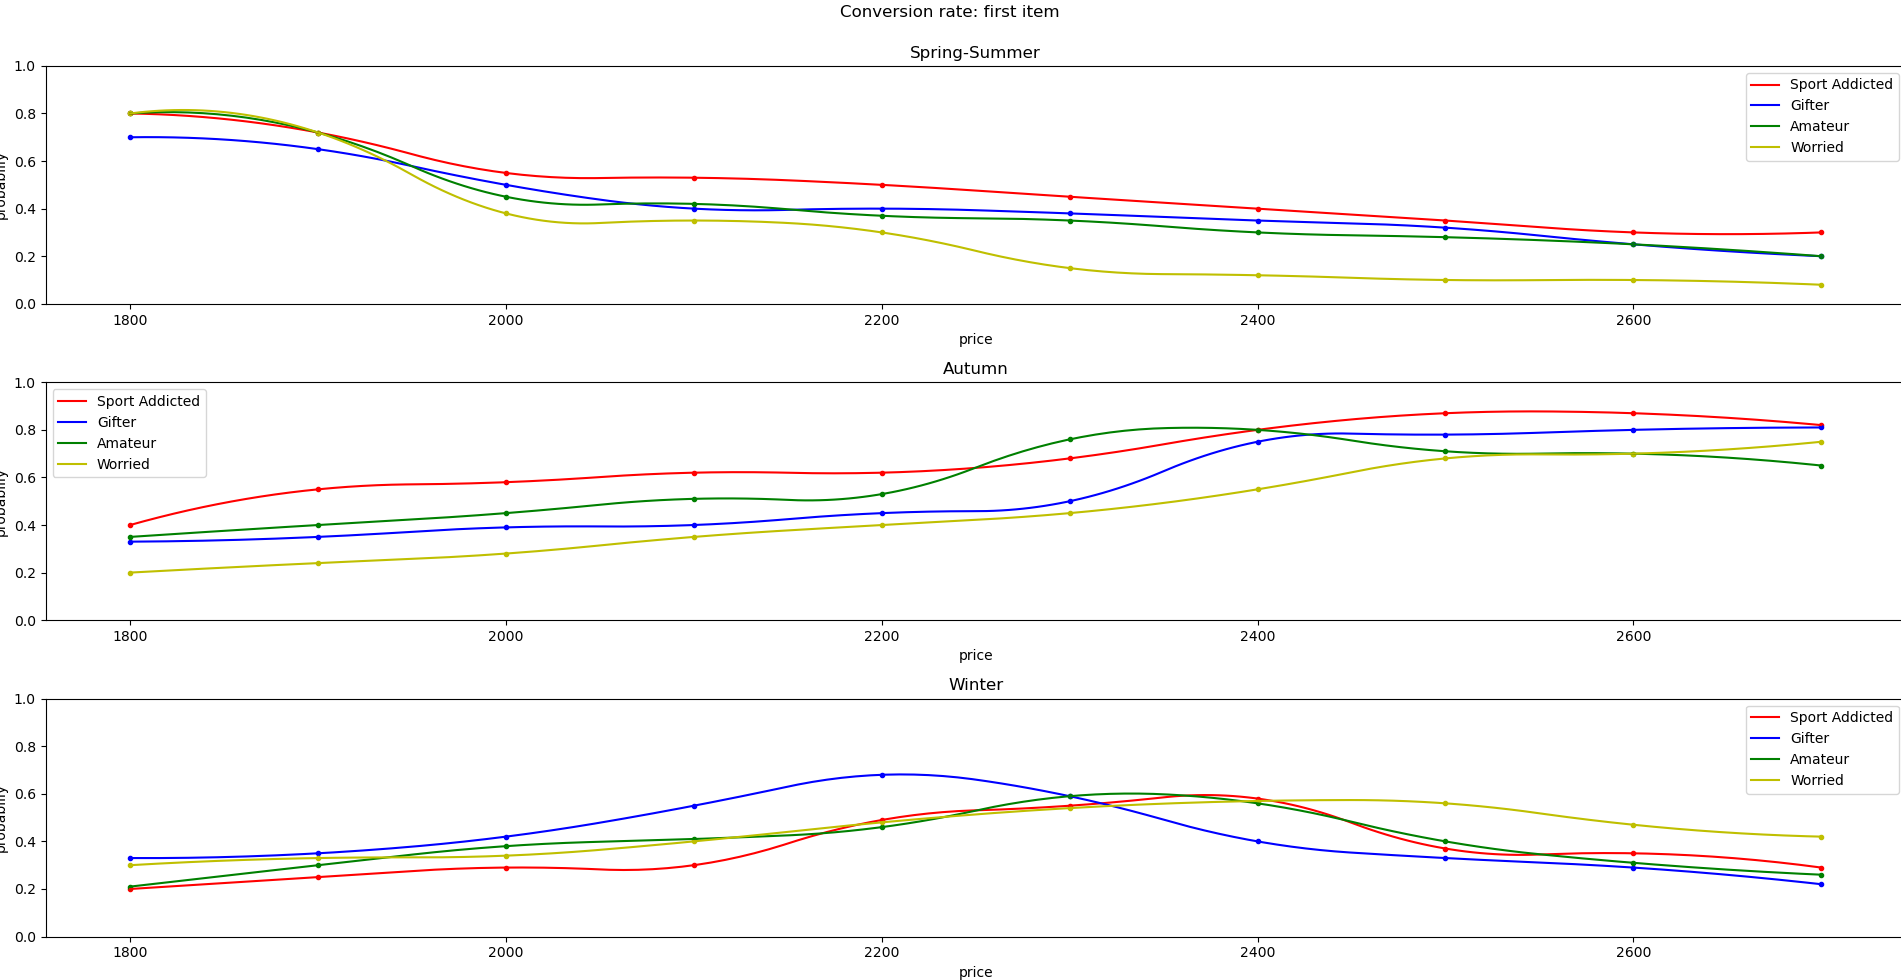
\includegraphics[scale=0.3]{Images/CR_fstItem}
\end{center}

\begin{center}
	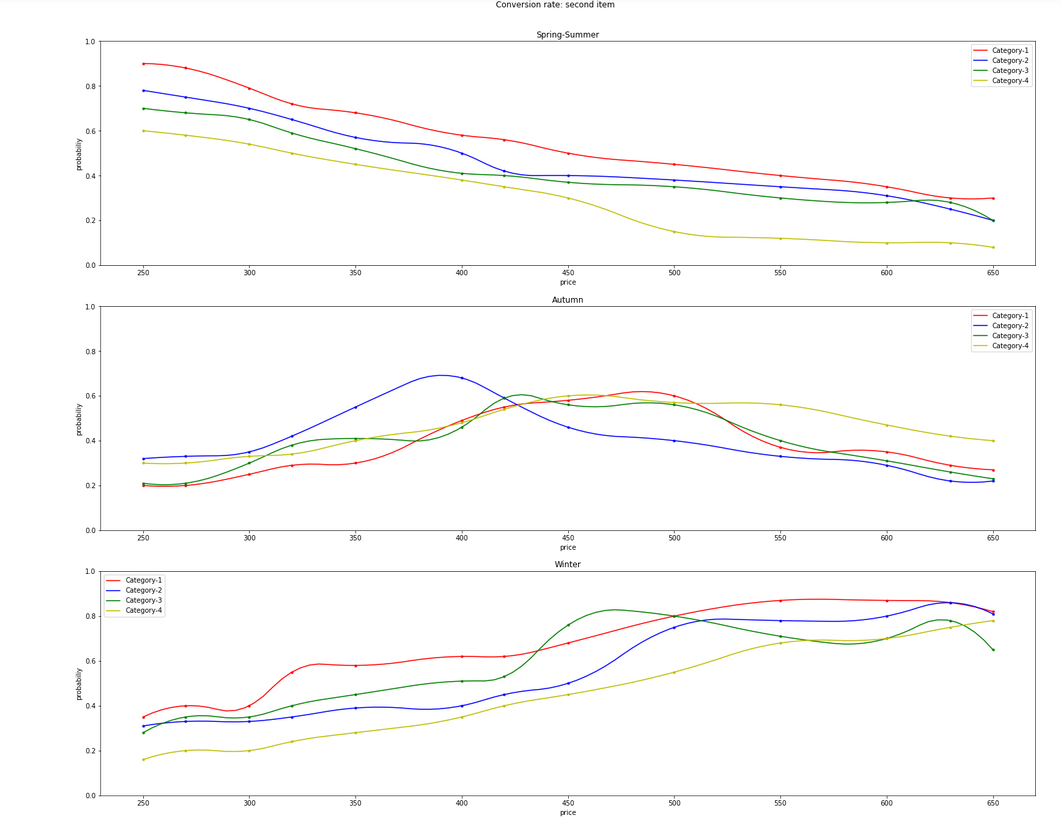
\includegraphics[scale=0.3]{Images/CR_scndItem}
\end{center}

\subsection*{Online Approach}
Our general approach for the online problem is to simulate the shop, day by day, generating the customers and emulating their behaviors, collecting the results and, according to the considered scenario and constraints, provide an optimal solution that maximize the reward.\\
Every day we retrieve the daily customer distribution per class using the previously presented random variable that model the daily customer distribution. Randomly we simulate the entry of a new customer, of which we know the category of belonging, in the shop. With an online approach we select the best price to be proposed to the client, in order to maximize the overall reward. The purchase is simulated with the previously presented random variable with a Bernulli distribution.
The second item is proposed to the client only if the first has been purchased. The price at which it is proposed is retrieved with an online matching approach that try to suggest which is the best discount to apply to the user in order to maximize the reward.\\
This procedure is repeated for all clients during the entire time horizon of 365 days. 
